% Bioinformatics Term Project -- Final Report
% Build:  tectonic reports/final_report_cpp_gnn.tex
%     or: pdflatex reports/final_report_cpp_gnn.tex   (run twice for the ToC)
\documentclass[11pt,a4paper]{article}

\usepackage[T1]{fontenc}
\usepackage[utf8]{inputenc}
\usepackage[a4paper,top=25mm,bottom=22mm,left=22mm,right=22mm]{geometry}
\usepackage{charter}
\usepackage[scaled=0.92]{helvet}
\usepackage{courier}
\usepackage{xcolor}
\usepackage{titlesec}
\usepackage{fancyhdr}
\usepackage{booktabs}
\usepackage{array}
\usepackage{multirow}
\usepackage{caption}
\usepackage{enumitem}
\usepackage{tikz}
\usepackage{microtype}
% Long identifiers such as BCEWithLogitsLoss overflow the margin in \texttt
% unless typewriter text is allowed to hyphenate.
\usepackage[htt]{hyphenat}
\usepackage[hidelinks]{hyperref}

\definecolor{navy}{HTML}{17405A}
\definecolor{tealx}{HTML}{13796D}
\definecolor{downr}{HTML}{B3402A}
\definecolor{bandg}{HTML}{EEF3F5}
\definecolor{rulec}{HTML}{C9D3D8}

% ---- headings: sans, navy sections, teal subsections (as in PR#3) ----
\titleformat{\section}{\sffamily\bfseries\large\color{navy}}{\thesection}{0.6em}{}
\titleformat{\subsection}{\sffamily\bfseries\normalsize\color{tealx}}{\thesubsection}{0.6em}{}
\titleformat{\subsubsection}{\sffamily\bfseries\small}{\thesubsubsection}{0.6em}{}
\titlespacing*{\section}{0pt}{1.6em}{0.6em}
\titlespacing*{\subsection}{0pt}{1.2em}{0.4em}

\pagestyle{fancy}
\fancyhf{}
\fancyhead[L]{\sffamily\footnotesize Bioinformatics Term Project}
\fancyhead[R]{\sffamily\footnotesize Final Report}
\fancyfoot[C]{\footnotesize\thepage}
\renewcommand{\headrulewidth}{0.4pt}

\captionsetup{font=small,labelfont={bf,sf},labelsep=colon,width=0.92\textwidth}
\setlist[itemize]{itemsep=2pt,topsep=3pt,parsep=0pt}

\newcommand{\up}[1]{\textcolor{tealx}{#1}}
\newcommand{\dn}[1]{\textcolor{downr}{#1}}
\newcommand{\code}[1]{\texttt{\small #1}}

\begin{document}

% =====================================================================
% TITLE PAGE
% =====================================================================
\begin{titlepage}
\thispagestyle{empty}
\begin{tikzpicture}[remember picture, overlay]
  \fill[navy] (current page.north west) rectangle ([yshift=-7.2cm]current page.north east);
  \fill[tealx] ([yshift=-7.2cm]current page.north west)
        rectangle ([yshift=-7.35cm]current page.north east);
  \node[anchor=north west, text width=15.5cm, align=left, inner sep=0pt]
    at ([xshift=2.2cm,yshift=-2.0cm]current page.north west) {%
      \color{white}\sffamily
      {\footnotesize B\,I\,O\,I\,N\,F\,O\,R\,M\,A\,T\,I\,C\,S\ \ T\,E\,R\,M\ \ P\,R\,O\,J\,E\,C\,T}\\[0.9em]
      {\bfseries\fontsize{21}{27}\selectfont Improving Long-Range Cell-Penetrating
       Peptide Prediction with Enhanced Graph Neural Networks}%
    };
\end{tikzpicture}

\vspace*{9.5cm}
\begin{center}
  {\sffamily\bfseries\fontsize{19}{23}\selectfont Final Report}\\[0.7em]
  \rule{0.5\textwidth}{0.4pt}\\[0.9em]
  {\large Is the Dataset, Not the Architecture, the Limiting Factor?}\\[0.35em]
  {\large A Controlled Two-Arm Experiment on a Merged MLCPP Dataset}
\end{center}

\vfill
\begin{center}
\fbox{\parbox{0.68\textwidth}{\vspace{2mm}
  \hspace{3mm}{\sffamily\bfseries Team Members}\\[2mm]
  \hspace*{3mm}\begin{tabular}{@{}r@{\hspace{1.5em}}p{6.2cm}r@{}}
    1. & Akkharachai Yongsuwankul & 6630357821\\
    2. & Apimook Sarovath        & 6631358621\\
    3. & Nasapon Pitoonmanit     & 6630078721\\
  \end{tabular}\hspace*{3mm}
\vspace{2mm}}}
\end{center}
\vspace*{1.5cm}
\end{titlepage}

% =====================================================================
\newpage
{\sffamily\bfseries\Large\color{navy}Contents}
\vspace{0.5em}
\renewcommand{\contentsname}{}
\vspace{-2.5em}
\tableofcontents
\newpage

% =====================================================================
\section{Further Development after Progress Report \#3}

\subsection{Continuation from Progress Report \#3}
Progress Report \#2 raised GraphSAGE message-passing depth from two layers to four and improved
independent-test MCC from 0.5963 to 0.6389. Progress Report \#3 tested whether that trend continued.
It did not. Extending GraphSAGE to six layers lowered MCC to 0.6101. A TransformerConv layer with four
attention heads and 11-dimensional bond features matched GraphSAGE-4 exactly on every threshold-based
metric at two layers (MCC 0.6389) and fell to 0.5807 at four layers, despite carrying $2.9\times$ the
parameters.

Four architectures spanning 332k to 1.15M parameters, two aggregation families and three depths all
arrived at essentially the same place. Progress Report \#3 concluded that architecture is not the
limiting factor, and listed as its first next step that the experiments should be repeated across
several seeds, because the differences were small enough to be run-to-run variation.

\subsection{Research Question}
If models that differ this much in capacity and in inductive bias plateau together, the plateau is more
likely a property of the data than of the models. The original CPP1708 training split contains only
1{,}497 peptides, with 187 for validation and 188 held out for testing. This report therefore asks:

\begin{center}
\colorbox{bandg}{\parbox{0.93\textwidth}{\vspace{1mm}\itshape
Does adding external cell-penetrating peptide data improve performance, and does the benefit depend on
the architecture?\vspace{1mm}}}
\end{center}

The second half of the question matters as much as the first. A single averaged number would hide the
possibility that extra data helps some architectures and harms others, which is what we in fact observe.

\subsection{Code Development}
Four additions were made to the repository. None of them change the model itself, so comparison with
Progress Reports \#2 and \#3 remains valid.

\begin{itemize}
  \sloppy % long code identifiers in this list would otherwise run into the margin
  \item \code{prepare\_merged\_dataset.py} pools every available source, removes duplicates by RDKit
  canonical SMILES, carves the shared holdout \emph{first} and only then builds the two training sets.
  It writes a \code{manifest.json} per arm recording split sizes and the required \code{pos\_weight}.
  It refuses to run if any peptide carries conflicting labels across sources, rather than silently
  choosing one.
  \item \code{graphcpp/lightning.py} gained \code{pos\_weight} support. The training loss is a weighted
  \code{BCEWith\-Logits\-Loss}; validation and test loss stay unweighted so they remain comparable between
  arms of different class balance.
  \item \code{main.py} gained \code{--pos\_weight} and \code{--results\_dir}, so the two arms write to
  separate result directories within one session.
  \item \code{pr4\_length\_delta.py} differences the two arms within each length bin. It verifies that
  both arms were evaluated on identical test peptides before computing anything, and exits with an error
  if they were not.
\end{itemize}

One defect in the Progress Report \#3 tooling was found and corrected while preparing this report. In
\code{evaluate\_pr3.py} the paired-analysis reference follows the first entry of \code{--models}, but the
printed heading, the two column names and the output filename all hard-coded ``SAGE-4''. The tables in
Section~\ref{sec:paired} are therefore computed against GraphSAGE-2, and the code now labels them with
the reference actually used.

\subsection{Controlled Experimental Protocol}
All ten training runs were executed in a single Kaggle session on one Tesla T4 GPU, using Python 3.10,
PyTorch 1.13.1+cu117, PyTorch Geometric 2.3.0, PyTorch Lightning 2.0.1, RDKit 2022.09.5 and DeepChem
2.7.1 --- the same software versions as Progress Reports \#2 and \#3. Every run uses seed 42, hidden
size 128, mean pooling, the topological-torsion fingerprint branch, Adam at learning rate 0.001 with a
cosine schedule, 100 epochs, batch size 512, and selects the checkpoint with the highest validation MCC.
The classification threshold is 0.5 throughout. Before training, a sanity check passed one real batch of
the 300 holdout graphs (51{,}063 atoms, 104{,}152 directed bonds) through all five architectures and
confirmed a finite loss from each.

% =====================================================================
\section{Dataset Construction}

\subsection{Sources and Deduplication}
Four sources were pooled: the original CPP1708 train, validation and test splits, and the MLCPP2
independent set~\cite{mlcpp}. Deduplication uses canonical SMILES rather than raw strings, because one
molecule has many valid SMILES spellings and raw string matching would leave duplicates in place. A
duplicate surviving into both the training set and the holdout would inflate every score reported here.

\begin{table}[h]
\centering\small
\begin{tabular}{@{}lrl@{}}
\toprule
\sffamily\bfseries\color{navy}Source & \sffamily\bfseries\color{navy}Rows & \sffamily\bfseries\color{navy}Role\\
\midrule
MLCPP2 independent set & 2{,}341 & new external data\\
CPP1708 train          & 1{,}497 & original\\
CPP1708 test           &    188 & original\\
CPP1708 validation     &    187 & original\\
\midrule
Pooled total           & 4{,}213 & \\
Duplicates removed     &    535 & zero label conflicts\\
\textbf{Unique peptides} & \textbf{3{,}678} & \textbf{used in this study}\\
\bottomrule
\end{tabular}
\caption{Pooled sources and the result of canonical-SMILES deduplication.}
\end{table}

Of the 2{,}341 MLCPP2 rows, 535 were already present in the original splits, leaving 1{,}806 genuinely
new peptides. No peptide appeared with conflicting labels in two sources, which is evidence that the two
datasets use a compatible definition of cell penetration and can legitimately be pooled.

\subsection{Two Arms Sharing One Holdout}
The design decision that makes this experiment interpretable is the order of operations. If each arm were
given its own test set, a change in score could be caused by the extra training data \emph{or} by the
change of test set, and the two causes could not be separated. The holdout is therefore drawn first, from
the deduplicated pool, and both training sets are built from what remains.

\begin{table}[h]
\centering\small
\begin{tabular}{@{}lrcrc@{}}
\toprule
& \multicolumn{2}{c}{\sffamily\bfseries\color{navy}Arm ORIGINAL} & \multicolumn{2}{c}{\sffamily\bfseries\color{navy}Arm MERGED}\\
\cmidrule(lr){2-3}\cmidrule(lr){4-5}
\sffamily\bfseries\color{navy}Split & Rows & Positive / Negative & Rows & Positive / Negative\\
\midrule
Train               & 1{,}272 & 636 / 636 & 3{,}078 & 748 / 2{,}330\\
Validation          &    300 & 150 / 150 &    300 & 150 / 150\\
Test (shared)       &    300 & 150 / 150 &    300 & 150 / 150\\
\midrule
Positive fraction, train & \multicolumn{2}{c}{50.0\,\%} & \multicolumn{2}{c}{24.3\,\%}\\
\code{pos\_weight} applied & \multicolumn{2}{c}{1.0000} & \multicolumn{2}{c}{3.1150}\\
\bottomrule
\end{tabular}
\caption{The two experimental arms. Validation and test splits are byte-identical between arms; only the
training data differs.}
\end{table}

Two independent guards enforce the shared holdout. The notebook compares the two arms' \code{val.csv} and
\code{test.csv} with \code{filecmp} before training begins, and \code{pr4\_length\_delta.py} re-checks
peptide identity, name and label alignment before computing any difference. Both reported identical files
for this run.

\subsection{Class Imbalance and the Weighted Loss}
The MLCPP2 independent set is approximately 93\,\% negative, so the merged training set is imbalanced:
748 positive against 2{,}330 negative. Two options were considered. Subsampling the negatives to restore a
50/50 balance would discard 1{,}582 real negative examples and grow the training set from 1{,}272 only to
1{,}496 rows --- a 12\,\% increase instead of 96\,\%. We rejected it: negative examples are information,
and realistic peptide screening is itself imbalanced, so a model trained on an artificially balanced set
is miscalibrated for its own task.

Instead the positive class is weighted in the training loss by
$\code{pos\_weight} = 2330/748 = 3.1150$. Because $748 \times 3.1150 = 2330$ exactly, the weighted
positive mass equals the negative mass, so the gradient signal is balanced while every real negative
example is retained. The \texttt{original} arm comes out exactly balanced at 636/636, so its
\code{pos\_weight} is 1.0 and its loss function is identical to that of Progress Reports \#2 and \#3.
Validation and test losses are never weighted.

% =====================================================================
\section{Experimental Results}
Ten training runs were performed: five architectures $\times$ two data arms. Each architecture evaluated
on the merged arm constitutes one additional experiment relative to Progress Report \#3, with
GraphSAGE-4 --- the Progress Report \#2 reference --- as the primary comparison.

\subsection{Overall Classification Performance}

\begin{table}[h]
\centering\footnotesize
\setlength{\tabcolsep}{4.5pt}
\begin{tabular}{@{}lrrrrrrr@{}}
\toprule
\sffamily\bfseries\color{navy}Model & \sffamily\bfseries\color{navy}Accuracy & \sffamily\bfseries\color{navy}MCC &
\sffamily\bfseries\color{navy}ROC-AUC & \sffamily\bfseries\color{navy}Precision & \sffamily\bfseries\color{navy}Recall &
\sffamily\bfseries\color{navy}F1 & \sffamily\bfseries\color{navy}Params\\
\midrule
\multicolumn{8}{@{}l}{\itshape Arm ORIGINAL --- trained on 1{,}272 original peptides}\\
GraphSAGE-2        & 0.7900 & 0.5822 & 0.8676 & 0.8175 & 0.7467 & 0.7805 & 332{,}546\\
GraphSAGE-4 (ref.) & 0.7833 & 0.5682 & 0.8608 & 0.8058 & 0.7467 & 0.7751 & 398{,}338\\
GraphSAGE-6        & 0.7933 & 0.5871 & 0.8625 & 0.7821 & 0.8133 & 0.7974 & 464{,}130\\
TransformerConv-2  & 0.7933 & 0.5869 & 0.8631 & 0.8014 & 0.7800 & 0.7905 & 707{,}330\\
TransformerConv-4  & 0.7767 & 0.5543 & 0.8636 & 0.7943 & 0.7467 & 0.7698 & 1{,}147{,}906\\
\midrule
\multicolumn{8}{@{}l}{\itshape Arm MERGED --- trained on 3{,}078 peptides, \code{pos\_weight} 3.115}\\
GraphSAGE-2        & 0.7667 & 0.5334 & 0.8581 & 0.7632 & 0.7733 & 0.7682 & 332{,}546\\
\textbf{GraphSAGE-4} & \textbf{0.8033} & \textbf{0.6068} & \textbf{0.8774} & 0.7974 & 0.8133 & \textbf{0.8053} & 398{,}338\\
GraphSAGE-6        & 0.7800 & 0.5612 & 0.8639 & 0.8000 & 0.7467 & 0.7724 & 464{,}130\\
TransformerConv-2  & 0.7867 & 0.5752 & 0.8740 & 0.8116 & 0.7467 & 0.7778 & 707{,}330\\
TransformerConv-4  & 0.7900 & 0.5858 & 0.8720 & 0.8372 & 0.7200 & 0.7742 & 1{,}147{,}906\\
\bottomrule
\end{tabular}
\caption{Independent-test performance on the shared 300-peptide holdout (threshold 0.5, best checkpoint
by validation MCC).}
\end{table}

The best result of the entire project is GraphSAGE-4 trained on merged data: MCC 0.6068 and ROC-AUC
0.8774. It is also the only configuration that improves on accuracy, MCC, ROC-AUC, recall and F1
simultaneously.

These numbers are \emph{not} directly comparable with the 0.6389 reported in Progress Reports \#2 and
\#3. That figure was measured on the original 188-peptide test set, whereas every number here is measured
on the new 300-peptide holdout, which had to be re-drawn so that both arms could share it. Within this
report all ten runs are measured on the same peptides, so the comparisons below are internally valid.

\subsection{Effect of the Merged Data per Architecture}
\label{sec:effect}

\begin{table}[h]
\centering\small
\begin{tabular}{@{}lrrrrr@{}}
\toprule
\sffamily\bfseries\color{navy}Model & \sffamily\bfseries\color{navy}MCC original &
\sffamily\bfseries\color{navy}MCC merged & \sffamily\bfseries\color{navy}$\Delta$ MCC &
\sffamily\bfseries\color{navy}$\Delta$ ROC-AUC & \sffamily\bfseries\color{navy}$\Delta$ Accuracy\\
\midrule
\textbf{GraphSAGE-4} & 0.5682 & 0.6068 & \up{$+0.0386$} & \up{$+0.0166$} & \up{$+0.0200$}\\
TransformerConv-4    & 0.5543 & 0.5858 & \up{$+0.0314$} & \up{$+0.0083$} & \up{$+0.0133$}\\
TransformerConv-2    & 0.5869 & 0.5752 & \dn{$-0.0117$} & \up{$+0.0109$} & \dn{$-0.0067$}\\
GraphSAGE-6          & 0.5871 & 0.5612 & \dn{$-0.0259$} & \up{$+0.0014$} & \dn{$-0.0133$}\\
GraphSAGE-2          & 0.5822 & 0.5334 & \dn{$-0.0488$} & \dn{$-0.0095$} & \dn{$-0.0233$}\\
\midrule
\textbf{Mean}        & 0.5757 & 0.5725 & \dn{$-0.0033$} & \up{$+0.0056$} & \dn{$-0.0020$}\\
\bottomrule
\end{tabular}
\caption{Change produced by the extra training data on the shared holdout. Positive values are
improvements.}
\end{table}

The mean change in MCC is $-0.0033$, which is no change at all. Taken alone, that number says the extra
data did nothing. The distribution says something more specific.

\begin{figure}[h]
\centering
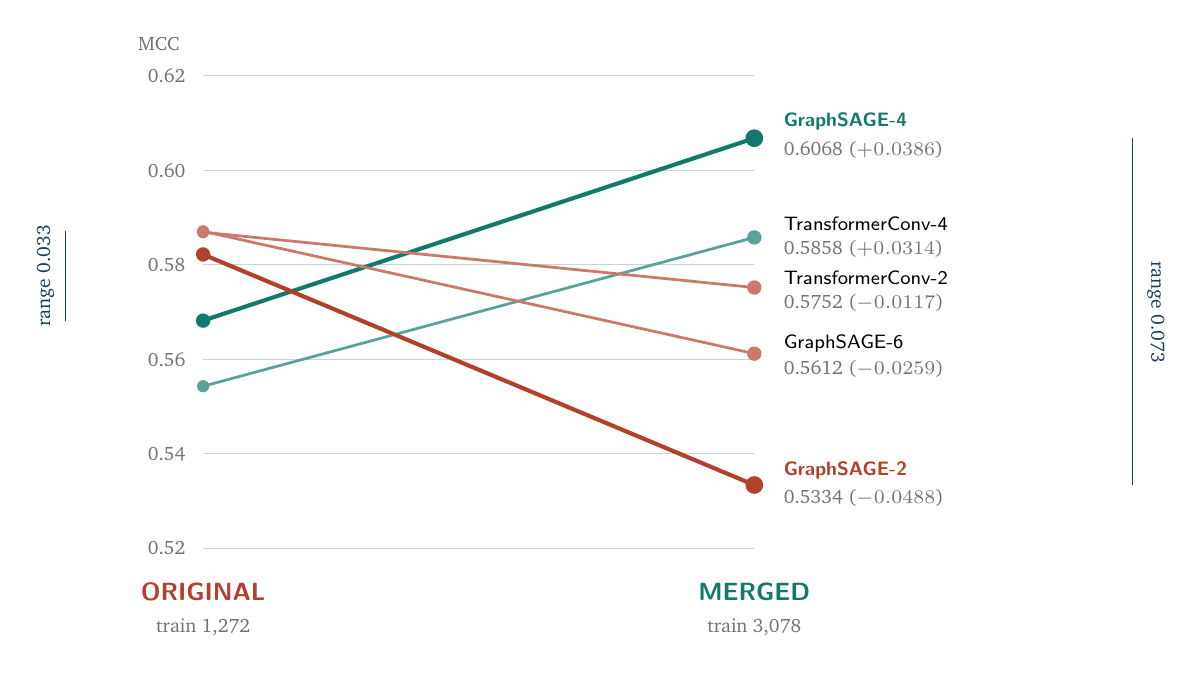
\begin{tikzpicture}[x=1cm,y=1cm]
  % grid: y = (MCC - 0.52) * 60
  \foreach \v/\yy in {0.52/0, 0.54/1.2, 0.56/2.4, 0.58/3.6, 0.60/4.8, 0.62/6.0} {
    \draw[rulec] (0,\yy) -- (7,\yy);
    \node[left, font=\scriptsize, text=black!55] at (-0.1,\yy) {\v};
  }
  \node[font=\scriptsize, text=black!55, anchor=south west] at (-0.95,6.2) {MCC};
  \node[font=\small\sffamily\bfseries, text=downr] at (0,-0.55) {ORIGINAL};
  \node[font=\small\sffamily\bfseries, text=tealx] at (7,-0.55) {MERGED};
  \node[font=\scriptsize, text=black!55] at (0,-1.0) {train 1,272};
  \node[font=\scriptsize, text=black!55] at (7,-1.0) {train 3,078};

  \draw[tealx, line width=1.5pt] (0,2.892) -- (7,5.208);
  \fill[tealx] (0,2.892) circle (2.6pt); \fill[tealx] (7,5.208) circle (3.2pt);
  \node[right, font=\scriptsize\sffamily\bfseries, text=tealx] at (7.25,5.42) {GraphSAGE-4};
  \node[right, font=\scriptsize, text=black!55] at (7.25,5.06) {0.6068 ($+0.0386$)};

  \draw[tealx!70, line width=1pt] (0,2.058) -- (7,3.948);
  \fill[tealx!70] (0,2.058) circle (2.2pt); \fill[tealx!70] (7,3.948) circle (2.6pt);
  \node[right, font=\scriptsize\sffamily] at (7.25,4.12) {TransformerConv-4};
  \node[right, font=\scriptsize, text=black!55] at (7.25,3.80) {0.5858 ($+0.0314$)};

  \draw[downr!70, line width=1pt] (0,4.014) -- (7,3.312);
  \fill[downr!70] (0,4.014) circle (2.2pt); \fill[downr!70] (7,3.312) circle (2.6pt);
  \node[right, font=\scriptsize\sffamily] at (7.25,3.44) {TransformerConv-2};
  \node[right, font=\scriptsize, text=black!55] at (7.25,3.12) {0.5752 ($-0.0117$)};

  \draw[downr!70, line width=1pt] (0,4.026) -- (7,2.472);
  \fill[downr!70] (0,4.026) circle (2.2pt); \fill[downr!70] (7,2.472) circle (2.6pt);
  \node[right, font=\scriptsize\sffamily] at (7.25,2.60) {GraphSAGE-6};
  \node[right, font=\scriptsize, text=black!55] at (7.25,2.28) {0.5612 ($-0.0259$)};

  \draw[downr, line width=1.5pt] (0,3.732) -- (7,0.804);
  \fill[downr] (0,3.732) circle (2.6pt); \fill[downr] (7,0.804) circle (3.2pt);
  \node[right, font=\scriptsize\sffamily\bfseries, text=downr] at (7.25,0.98) {GraphSAGE-2};
  \node[right, font=\scriptsize, text=black!55] at (7.25,0.64) {0.5334 ($-0.0488$)};

  % kept clear of the y-axis numbers, which run from about x=-1.0 to x=-0.1
  \draw[navy] (-1.75,2.892) -- (-1.75,4.026);
  \node[font=\scriptsize, text=navy, rotate=90] at (-2.0,3.46) {range 0.033};
  \draw[navy] (11.8,0.804) -- (11.8,5.208);
  \node[font=\scriptsize, text=navy, rotate=-90] at (12.1,3.0) {range 0.073};
\end{tikzpicture}
\caption{MCC of each architecture on the shared holdout. On the original data all five models lie within
a band of 0.033; on the merged data the band widens to 0.073. The mean barely moves, but the models
separate.}
\end{figure}

On original data the five architectures span MCC 0.5543 to 0.5871, a range of 0.0328 --- they are nearly
indistinguishable, which is the Progress Report \#3 finding restated on a larger holdout. On merged data
they span 0.5334 to 0.6068, a range of 0.0734, more than twice as wide. The extra data did not raise the
group; it separated it.

The direction of that separation follows capacity. The two models that gain are GraphSAGE-4 and
TransformerConv-4; the model that loses most is GraphSAGE-2, the smallest at 332{,}546 parameters and two
message-passing layers. The epoch at which each run reached its best validation MCC supports this
reading: on merged data GraphSAGE-2 peaked at epoch 17 and then degraded, while GraphSAGE-4 peaked at
epoch 65 and TransformerConv-2 at epoch 72. The larger models were still extracting signal from the
additional examples long after the smallest had stopped.

\subsection{Performance by Peptide-Length Range}
The length bins follow the non-overlapping interpretation used in Progress Reports \#2 and \#3. Because
the holdout is shared, the class composition of every bin is identical for all ten runs.

\begin{table}[h]
\centering\footnotesize
\setlength{\tabcolsep}{5pt}
\begin{tabular}{@{}lrrrrrrrr@{}}
\toprule
\sffamily\bfseries\color{navy}Range & \sffamily\bfseries\color{navy}N & \sffamily\bfseries\color{navy}CPP &
\sffamily\bfseries\color{navy}Paper~\cite{graphcpp} & \sffamily\bfseries\color{navy}SAGE-2 &
\sffamily\bfseries\color{navy}SAGE-4 & \sffamily\bfseries\color{navy}SAGE-6 &
\sffamily\bfseries\color{navy}TC-2 & \sffamily\bfseries\color{navy}TC-4\\
\midrule
11--16 & 88 & 58 & 0.769 & \up{$+0.011$} & \up{$+0.046$} & \dn{$-0.046$} & \dn{$-0.023$} & \up{$+0.011$}\\
16--22 & 95 & 49 & 0.781 & \dn{$-0.032$} & \up{$+0.032$} & \dn{$-0.011$} & \dn{$-0.011$} & \dn{$-0.011$}\\
22--27 & 37 & 13 & 0.875 & \dn{$-0.027$} & \up{$+0.027$} & $0.000$ & $0.000$ & $0.000$\\
27--33 & 49 & 17 & 0.765 & \dn{$-0.041$} & \dn{$-0.041$} & $0.000$ & \dn{$-0.020$} & \up{$+0.041$}\\
33--39 & 24 & 10 & 0.583 & \dn{$-0.042$} & $0.000$ & \up{$+0.042$} & \up{$+0.083$} & \up{$+0.083$}\\
39--44 &  5 &  2 & 0.500 & \dn{$-0.200$} & $0.000$ & $0.000$ & $0.000$ & $0.000$\\
outside 11--44 & 2 & 1 & --- & $0.000$ & $0.000$ & $0.000$ & $0.000$ & $0.000$\\
\midrule
\textbf{Overall} & 300 & 150 & --- & \dn{$-0.023$} & \up{$+0.020$} & \dn{$-0.013$} & \dn{$-0.007$} & \up{$+0.013$}\\
\bottomrule
\end{tabular}
\caption{Accuracy change (merged $-$ original) within each length range. Bin composition is identical
across all runs by construction.}
\end{table}

An ``outside 11--44'' row is reported explicitly. The paper's bins do not cover every peptide in this
holdout, and without that row the bin counts would not sum to 300, so a reader could not tell that two
peptides had been excluded from the length analysis.

GraphSAGE-4 is the only model that improves in the three shortest bins, which together hold 220 of the
300 holdout peptides: $+0.046$, $+0.032$ and $+0.027$ accuracy. Its one loss is in the 27--33 bin at
$-0.041$, which is two peptides.

The two longest bins must be read with care, and we report them only because Progress Reports \#2 and \#3
did. The 33--39 bin holds 24 peptides, so one peptide is 4.2 percentage points; the $+0.083$ accuracy and
$+0.172$ MCC recorded there for both TransformerConv variants amount to two peptides changing class. The
39--44 bin holds five peptides, so the $-0.200$ for GraphSAGE-2 is one peptide. These are not findings.
The long-peptide weakness that originally motivated this project remains unresolved, and this holdout is
too small in that region to resolve it.

\subsection{Ranking Quality versus Decision Threshold}
ROC-AUC and MCC disagree in Table~3, and the disagreement is systematic rather than random. ROC-AUC
improves in four of the five architectures (mean $+0.0056$) while MCC at threshold 0.5 does not (mean
$-0.0033$).

The two metrics measure different things. ROC-AUC is threshold-free: it asks whether the model ranks
penetrating peptides above non-penetrating ones at \emph{any} cut. MCC in this report is measured at a
fixed cut of 0.5. A consistent gain in the first with no gain in the second is the signature of a model
that has learned to order its inputs better while its probability scale has shifted.

That shift has an identifiable cause. The merged arm trains with \code{pos\_weight} 3.115, which by design
pushes predicted probabilities for the positive class upward relative to an unweighted model. The
threshold inherited from Progress Report \#2 is therefore no longer the operating point that maximises
MCC for the merged arm. The improvement in ranking is real and measurable; the fixed threshold conceals
part of it. Section~\ref{sec:next} proposes the inexpensive experiment that would quantify how much.

\subsection{Paired Same-Peptide Analysis}
\label{sec:paired}
Because all runs are evaluated on identical peptides, predictions can be compared one peptide at a time.
The reference here is GraphSAGE-2, the first entry passed to \code{--models}.

\begin{table}[h]
\centering\small
\begin{tabular}{@{}lrrrrrr@{}}
\toprule
& \multicolumn{3}{c}{\sffamily\bfseries\color{navy}Arm ORIGINAL} & \multicolumn{3}{c}{\sffamily\bfseries\color{navy}Arm MERGED}\\
\cmidrule(lr){2-4}\cmidrule(lr){5-7}
\sffamily\bfseries\color{navy}Model & Fixed & Broken & Net & Fixed & Broken & Net\\
\midrule
\textbf{GraphSAGE-4} &  3 &  5 & \dn{$-2$} & 18 &  7 & \up{$+11$}\\
GraphSAGE-6          & 10 &  9 & \up{$+1$} & 18 & 14 & \up{$+4$}\\
TransformerConv-2    &  7 &  6 & \up{$+1$} & 15 &  9 & \up{$+6$}\\
TransformerConv-4    &  4 &  8 & \dn{$-4$} & 19 & 12 & \up{$+7$}\\
\bottomrule
\end{tabular}
\caption{Paired comparison against GraphSAGE-2 over all 300 holdout peptides. \emph{Fixed}: reference
wrong, model correct. \emph{Broken}: reference correct, model wrong. Net $=$ Fixed $-$ Broken.}
\end{table}

This table is the clearest single piece of evidence for the separation described in
Section~\ref{sec:effect}. On the original data every model sits within four peptides of GraphSAGE-2 and
the net corrections scatter around zero, two positive and two negative. On the merged data all four net
corrections are positive and substantially larger, with GraphSAGE-4 correcting eleven peptides net. The
same five architectures that were interchangeable on 1{,}272 training peptides are clearly ordered on
3{,}078.

% =====================================================================
\section{Discussion, Limitations, and Conclusions}

\subsection{Findings across Progress Reports \#2 to \#4}
\textbf{Depth helps, then stops helping.} Progress Report \#2 showed that going from two to four
message-passing layers improved MCC from 0.5963 to 0.6389. Progress Report \#3 showed that six layers
reversed the gain. Four layers remains the best depth tested, consistent with over-smoothing: beyond a
certain number of rounds, every atom's representation converges toward the graph average and
peptide-specific structure is lost.

\textbf{Attention did not beat fixed-weight aggregation.} TransformerConv was given the bond features
that GraphSAGE ignores and still did not exceed it, at either depth, in either report. PyTorch Geometric's
TransformerConv attends only over bonded neighbours, so it changes \emph{how} neighbour information is
weighted, not \emph{how far} information travels. It is not a global graph transformer, and the
long-peptide limitation it was introduced to address is a question about distance, not about weighting.

\textbf{More data is not a free improvement either.} Nearly doubling the training set changed mean MCC by
$-0.0033$. Both of the obvious levers --- a bigger model and a bigger dataset --- have now been pulled,
and neither moved the average.

\textbf{What the data actually did was separate the architectures.} The spread in MCC more than doubled,
from 0.033 to 0.073, and the ordering became consistent across the overall table, the length bins and the
paired analysis. GraphSAGE-4 improves on every metric; GraphSAGE-2 degrades on every metric. This is the
most useful result in the report, and it is invisible in the average.

\subsection{Limitations}
\begin{itemize}
  \item \textbf{No new peptide reached the holdout.} RDKit's \code{Chem.MolToSequence()} returns an empty
  string for a molecule parsed from plain SMILES without residue information. The original splits carry a
  \code{sequence} column and passed; the MLCPP2 rows do not, so all 1{,}806 new peptides were assigned to
  training only. This experiment therefore measures whether extra data helps \emph{on the original data
  distribution}. It cannot support any claim about generalisation to the MLCPP distribution.
  \item \textbf{Single seed.} Every number comes from one run at seed 42. Progress Report \#3 raised this
  same limitation and it remains unaddressed. Differences of $\pm 0.05$ MCC may lie within run-to-run
  variation, which means the central comparison of Section~\ref{sec:effect} --- $+0.0386$ for GraphSAGE-4
  against $-0.0488$ for GraphSAGE-2 --- is suggestive rather than established.
  \item \textbf{Small bins in the length analysis.} Two of six bins hold 24 and 5 peptides. Per-bin values
  there are reported for continuity with earlier reports and should not be interpreted individually.
  \item \textbf{All new negatives come from one source.} 1{,}694 of the 1{,}806 new peptides are negative
  and all originate from MLCPP2. A model may learn that peptides resembling MLCPP2 negatives are negative,
  which is a property of the dataset rather than of membrane biology.
  \item \textbf{Positives remain scarce.} The merge added only 112 positive examples, taking the count
  from 636 to 748. The scarce resource in this problem is confirmed cell-penetrating peptides, and the
  merge did not meaningfully relieve it.
\end{itemize}

\subsection{Conclusions}
Across three progress reports this project tested two hypotheses about why GraphCPP plateaus, and rejected
both in their simple form. Architecture is not the bottleneck: depth beyond four layers and
attention-based aggregation both failed to improve on GraphSAGE-4. Dataset size is not the bottleneck
either, at least not on its own: a 96\,\% larger training set moved mean MCC by $-0.0033$.

What the experiment does establish is an interaction between the two. Additional data is only useful to a
model with the capacity to absorb it, and the same additional data actively harms the smallest model
tested. The practical recommendation that follows is that GraphSAGE-4 should remain the reference
configuration, and that it should be trained on the merged dataset, where it reaches the best result
obtained in this project: MCC 0.6068 and ROC-AUC 0.8774 on a balanced 300-peptide holdout.

\subsection{Next Steps}
\label{sec:next}
\begin{itemize}
  \item \textbf{Establish the noise floor.} Repeat the GraphSAGE-4 comparison over at least three seeds in
  both arms and report mean $\pm$ standard deviation. At the measured cost of roughly 2--5 minutes per run
  on a T4, this is about 25 minutes of compute and it determines whether Section~\ref{sec:effect} describes
  a real effect. This is the single highest-value follow-up.
  \item \textbf{Sweep the decision threshold.} The saved per-peptide prediction files already contain the
  probabilities, so this requires no retraining. Finding the MCC-maximising threshold per arm would show
  how much of the ROC-AUC gain is recoverable.
  \item \textbf{Recover sequences for the MLCPP peptides} so that they can enter the holdout, which would
  turn the central limitation above into a testable claim about generalisation.
  \item \textbf{Address distance rather than weighting.} The long-peptide weakness motivated the attention
  experiments, but local attention does not change the receptive field. A virtual node, or a graph
  transformer with positional encodings, would.
  \item \textbf{Obtain more positive examples,} which remain the binding constraint at 748.
\end{itemize}

% =====================================================================
\subsection*{Summary of the Final Report}
\addcontentsline{toc}{section}{Summary of the Final Report}

\begin{table}[h]
\centering\small
\begin{tabular}{@{}p{0.27\textwidth}p{0.66\textwidth}@{}}
\toprule
\sffamily\bfseries\color{navy}Rubric item & \sffamily\bfseries\color{navy}Evidence provided in this report\\
\midrule
(1) At least two additional experimental results &
Five additional experiments, one per architecture, each trained on the merged dataset and compared against
its own original-data counterpart on a shared holdout: GraphSAGE-2 ($\Delta$MCC $-0.0488$), GraphSAGE-4
($+0.0386$), GraphSAGE-6 ($-0.0259$), TransformerConv-2 ($-0.0117$) and TransformerConv-4 ($+0.0314$); ten
training runs in total. Reported overall (Tables 3--4, Figure 1), by peptide-length range (Table 5) and per
peptide (Table 6). Supporting development: a merged dataset of 3{,}678 deduplicated peptides (Tables 1--2)
and \code{pos\_weight} support for imbalanced training (Section 2.3).\\
\addlinespace
(2) Discussion and summary of all results &
Section 4.1 draws the findings of Progress Reports \#2, \#3 and \#4 together: depth helps to four layers
then reverses, attention does not beat fixed-weight aggregation, more data does not raise the mean, and the
real effect of more data is to separate architectures by capacity. Section 4.2 states five limitations,
including the holdout composition and the single seed carried over from Progress Report \#3. Section 4.3
gives the conclusions and the recommended configuration; Section 4.4 gives costed next steps.\\
\bottomrule
\end{tabular}
\end{table}

% =====================================================================
\begin{thebibliography}{9}
\footnotesize
\bibitem{graphcpp} A. Imre, B. Balogh, and I. M\'andity, ``GraphCPP: The new state-of-the-art method for
cell-penetrating peptide prediction via graph neural networks,'' \emph{British Journal of Pharmacology},
vol.~182, no.~3, pp.~495--509, 2025. doi:10.1111/bph.17388.
\bibitem{sage} W. Hamilton, Z. Ying, and J. Leskovec, ``Inductive representation learning on large
graphs,'' in \emph{Advances in Neural Information Processing Systems}, vol.~30, 2017.
\bibitem{transformerconv} Y. Shi, Z. Huang, S. Feng, H. Zhong, W. Wang, and Y. Sun, ``Masked label
prediction: Unified message passing model for semi-supervised classification,'' in \emph{Proceedings of
the 30th International Joint Conference on Artificial Intelligence (IJCAI)}, 2021, pp.~1548--1554.
\bibitem{pyg} M. Fey and J. E. Lenssen, ``Fast graph representation learning with PyTorch Geometric,'' in
\emph{ICLR Workshop on Representation Learning on Graphs and Manifolds}, 2019.
\bibitem{mlcpp} B. Manavalan \emph{et al.}, ``MLCPP 2.0: An updated cell-penetrating peptides and their
uptake efficiency predictor,'' \emph{Journal of Molecular Biology}, 2022. Data obtained from
\texttt{thegleelab.org/MLCPP}.
\end{thebibliography}

\end{document}
